\documentclass{article}
\usepackage{tikz}
\usepackage{pgfplots}
\pgfplotsset{compat=newest} % Allows to place the legend below plot
\usetikzlibrary{patterns}

%The variables to plot the graph
\newcommand\cpRoof{6.6}
\newcommand\xATcpRoof{1.11902991387417}
\newcommand\slopeBW{5.9}
\newcommand\designCI{1.7}
\newcommand\myXmax{1000}
\newcommand\myYmax{5000}
\newcommand\cpWithMaxScaling{5606.72660524781}
\newcommand\peakTheoBWGBps{10.4}
\newcommand\designCP{6.6}

\begin{document}

\begin{center}
%-------------------------------------------------
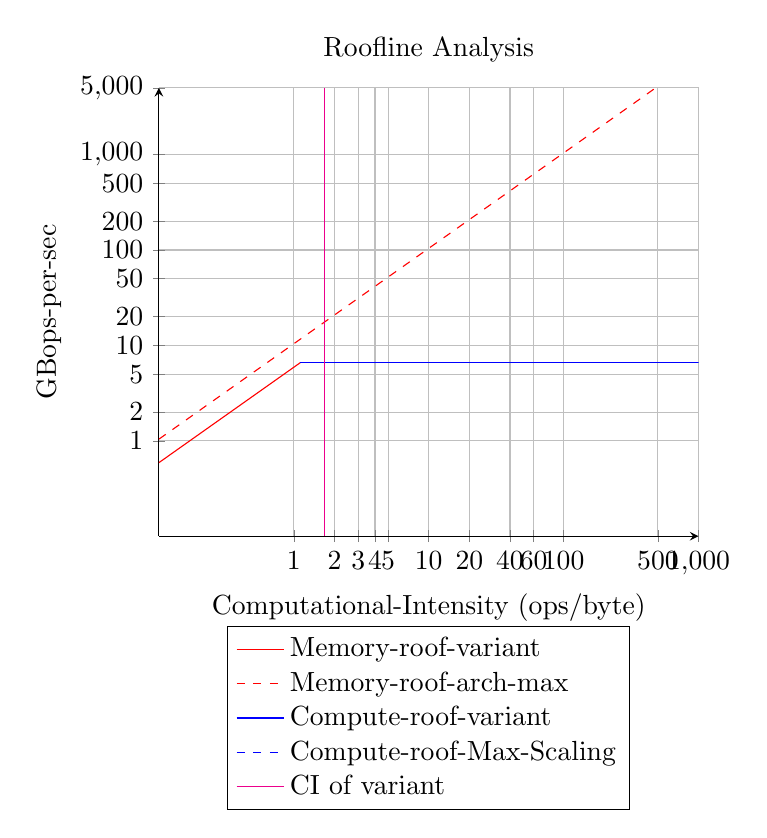
\begin{tikzpicture}
     
\begin{loglogaxis}[
    axis lines = left,
    xlabel = Computational-Intensity (ops/byte),
    ylabel = GBops-per-sec,
    title  = Roofline Analysis,
    log ticks with fixed point,
    xtick={0,1,2,3,4,5,10,20,40,60,100,500,1000},
    ytick={0,1,2,5,10,20,50,100,200,500,1000,5000},
        ymax=\myYmax,
    xmax=\myXmax,
    xmin=0.1,
    ymin=0.1,
    grid=major,
    legend style = {
            at = {(0.5,-0.2)},
            legend columns=1,
            legend cell align=left,
            anchor = north
    }        
]

%The Memory-bound region (sust BW for this variant)
\addplot [
    domain=0.1:\xATcpRoof, 
    samples=100, 
    color=red,
]
{\slopeBW*x};
\addlegendentry{Memory-roof-variant}


%The Memory-bound region (peak BW of archtitecture)
\addplot [
    domain=0.1:\myXmax, 
    samples=100, 
    color=red,
    dashed,
]
{\peakTheoBWGBps*x};
\addlegendentry{Memory-roof-arch-max}

%The compute-bound region
\addplot [
    domain=\xATcpRoof:\myXmax, 
    samples=100, 
    color=blue,
    ]
    {\cpRoof};
\addlegendentry{Compute-roof-variant}

%Theoretical maximum CP with scaling
\addplot [
    domain=0.1:\myXmax, 
    samples=100, 
    color=blue,
    dashed,
    ]
    {\cpWithMaxScaling};
\addlegendentry{Compute-roof-Max-Scaling} 
 

%The Performance of this variant (vertical line at CI)
\addplot [
    domain=0.1:\myXmax, 
    samples=100, 
    color=magenta,
    ]
    coordinates {(\designCI,0.1)(\designCI,\myYmax)};
\addlegendentry{CI of variant}
 
\end{loglogaxis}    
    
\end{tikzpicture}
\end{center}

\end{document}